\label{sec:charakterbogen}\begin{quote}
    Ach ich darf mein Leben gar nicht für die Punkte opfern?
\end{quote}
\subsection{Allgemeine Daten}

Hierbei sei erst einmal gesagt, dass das endgültige Layout des Charakterbogens noch nicht fertig ist (und ich gerne Designs/Zeichnungen von euch darin einbaue um das Ganze aufzuhübschen \Laughey) und ihr deswegen hier nur pragmatische Darstellungen der jeweiligen Sektion seht, die nur aus semantischer Sicht so übernommen werden.

\index{Punkte}Wichtig ist, dass es diesmal \index{Punkte!Spezifisch (\SP)}spezifische (\SP{}) und \index{Punkte!Global/Magisch (\GP)}globale (\GP{}) Punkte gibt. \SP{} sind an eine Fertigkeiten-Gruppe gebunden. \SP{} können \(4:1\) in \GP{} umgewandelt und damit auch in anderen Gruppen eingesetzt werden (\GP{} sind allerdings nicht mehr Wert, die einzige Ausnahme hiervon ist die Magie\ldots).% TODO: link Magie

\paragraph{Allgemeine Metadaten}
\label{par:charMeta}\begin{sccenter}
    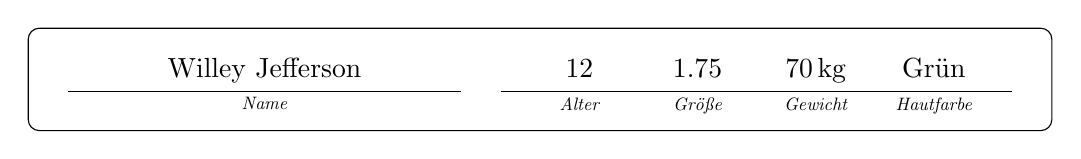
\begin{tikzpicture}[lc/.style={below,scale=0.65,font=\itshape}]
        \draw[rounded corners] (0,0) rectangle ++(13,1.3);
        \draw (0.5,0.5) -- ++(5,0) node[lc,midway] {Name} node[above=-0.215em,midway] {\strut{Willey Jefferson}};
        \draw (6,0.5) -- ++(6.5,0);
        \foreach[count=\i] \a/\b in {12/Alter,1.75/Größe,70\,kg/Gewicht,Grün/Hautfarbe} {
            \node[lc] at(7+1.5*\i-1.5,0.5) {\b}; 
            \node[above=-0.215em] at(7+1.5*\i-1.5,0.5) {\strut\a}; 
        }
    \end{tikzpicture}
\end{sccenter}
Die Daten, die dort eingetragen werden sollen, sollten ohne große Erklärung funktionieren. Deswegen hopp hopp, und weiter geht die Reise\ldots

\paragraph{Die Lebensversicherung}
\begin{wrapfigure}[4]{r}{0.375\linewidth}
    \vspace*{-0.75\topsep}\centering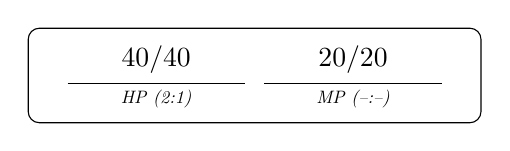
\begin{tikzpicture}[lc/.style={below,scale=0.65,font=\itshape}]
        \draw[rounded corners] (0,0) rectangle ++(5.75,1.2);
        \draw (0.5,0.5) -- ++(2.25,0) node[lc,midway] {HP (2:1)} node[above,midway] {40/{\smaller40}};
        \draw (3,0.5) -- ++(2.25,0) node[lc,midway] {MP (--:--)} node[above,midway] {20/{\smaller20}};
    \end{tikzpicture}
\end{wrapfigure}
Erstmal zu den \imp{Lebenspunkten (HP)}: 
Ihr startet mit 40, was nach verhältnismäßig wenig klingt aber schon ganz ordentlich ist im Verhältnis zum allgemeinen Schadenssystem. % TODO: LinK
Die Kosten für Leben betragen \(2:1\) und können aus allen anderen Gruppen zusammengespart werden. Der Verkaufspreis ist invertiert, ein Lebenspunkt liefert also zwei Fertigkeitenpunkte (\SP).
Die Lebenspunkte dürfen durch das verkaufen nicht auf oder unter Null gesetzt werden. Weniger Lebenspunkte werden aber auch hart bestraft\ldots

Eure Lebenspunkte sind den folgenden Regeln unterworfen:
\begin{itemize}
    \item \label{char:createNew}Fällt die Anzahl der Lebenspunkte aus einem beliebigen Grund auf oder unter \(0\) so scheidet der Charakter umgehend aus. In diesem Fall ist ein neuer Charakter zu erstellen, dessen Level zwei unter dem des bisher niedrigsten Gruppenlevels ist\footnote{Das Level kann über diese Mechanik nicht unter 1 gesetzt werden.}.
    \item Verursacht ein Angriff mindestens so viel Schaden wie die Hälfte der aktuellen Lebenspunkte, so ist eine Probe zu werfen (hier erscheint eine Referenz, sobald es diese Probe gibt). % TODO: link
    \item Fällt die Anzahl der Lebenspunkte unter 5, so gilt der Charakter als \imp{schwer verwundet} und kann eigenhändig keine Aktionen wie laufen, oder gar kämpfen durchführen.
    \item Jegliche Form von Heilung (egal ob magisch oder physisch) lässt sich für jede Wunde nur einmal pro Tag\footnote{Solche Begrenzungen setzen wir lose auf \say{alle \(24\)} Stunden, nicht das einer um Mitternacht direkt zwei Bandagen anbringen möchte.} anwenden.
    \item \index{Schlaf}Eine vom Spielmeister als \say{angenehm} eingestufte Nacht (in der geschlafen wurde) stellt \(\dice{1}{6} + 1\) Leben wieder her, sofern am Tag mindestens einmal am Tag gegessen wurde. Es steht dem Spielmeister frei, Schaden für das Unterlassen einer Nahrungsaufnahme zu verteilen.
\end{itemize}

Die \imp{Manapunkte (MP)} sind auf 20 beschränkt. Das Limit kann weder durch \SP/\GP{}, noch durch einen Levelaufstieg verändert werden.
Es existieren Gegenstände und Tier die selbst Mana innehaben und so zum wiederauffüllen verwendet werden können. Der Pool ist für den Anwender aber stets auf 20 eingegrenzt\footnote{So ist auch Magie in die beliebig viele Manapunkte investiert werden können auf maximal 20 Manapunkte beschränkt. Weitere \say{Manapunkte} können aber durch die gegebenen Regeln aufgebracht werden}. Für die Manapunkte gelten die folgenden Regeln:
\begin{itemize}
    \item Fällt das Mana, aus irgendeinem Grund, auf 0, so schließt dies nicht aus weiter Magie einzusetzen. Für je einen Lebenspunkte kann je ein weiterer Manapunkt investiert werden. So ist es auch möglich weiter zu zaubern, wenn der Mana-Pool aufgebraucht ist. Ein Magieanwender kann durch diese Mechanik zu Tode kommen.
    \item Schlaf generiert \emph{keine} Manapunkte.
    Magier können anstelle zu Schlafen auch \index{Meditation}\imp{Meditieren} und erhalten \(\dice{1}{4} + 1\) Manapunkte für eine \say{angnehme Nacht} zurück.
\end{itemize}

\paragraph{Level}
\begin{wrapfigure}[4]{r}{0.375\linewidth}
    \vspace*{-0.75\topsep}\centering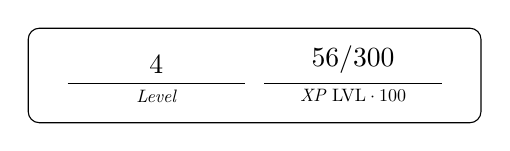
\begin{tikzpicture}[lc/.style={below,scale=0.65,font=\itshape}]
        \draw[rounded corners] (0,0) rectangle ++(5.75,1.2);
        \draw (0.5,0.5) -- ++(2.25,0) node[lc,midway] {Level} node[above,midway] {4};
        \draw (3,0.5) -- ++(2.25,0) node[lc,midway] {XP \(\mathrm{LVL} \cdot 100\)} node[above,midway] {56/{\smaller300}};
    \end{tikzpicture}
\end{wrapfigure}
Ein Charakter startet auf \imp{Level (LVL)} 1, sofern er nicht durch die \say{\link[char:createNew]{Neuerstellungsmechanik}} auf einem höheren Level beginnt.
Die \imp{Erfahrungspunkte (XP)} beginnen in jedem Falle bei \(0\).
Um ein Level aufzusteigen werden jeweils \(\mathrm{LVL} \cdot 100\) Erfahrungspunkte benötigt.
Um von Level 1 auf Level 2 aufzusteigen werden also 100, um von Level 2 auf Level 3 aufzusteigen werden 200 Erfahrungspunkte benötigt, und so weiter\ldots

Für den \imp{Levelaufstieg} von Level 1 auf Level 2 werden \SP[6] pro Kategorie und \GP[3] vergeben.
Jeder Aufstieg darüber wird mit \SP[6] in jeder Kategorie und \GP[4] vergütet.

\subsection{Ausrüstung}

Zusätzlich zu eurem super duper gezeichneten \imp{Bild} des Charakters\footnote{An das Bild ist eine hohe Erwartungshaltung gerichtet ist, schließlich soll das Verlieren eines charakters ja auch richtig weh tun \Winkey.} geht es nun einmal um die \imp{Ausrüstung} welches sein Antlitz teils überdeckt.
Auch wenn es hier etliche Segmente gibt, braucht ihr nicht für jede ein eigenes Rüstungsteil. Ihr könnt euch die \say{Deko}-Kleidung aussuchen. Diese Kleidung hat aber
keine Werte (ist also wirklich nur kosmetischer Natur) und hilft auch in Debatten wie \say{Aber schau mal auf dem Bild trägt der eindeutig ein Jetpack} nicht weiter.
Jeder der folgenden Slots kann mit einem Element/Kleidungsstück belegt werden welches
Rüstungspunkte und sogar weitere Vorteile mit sich bringen mag. Solche Gegenstände gilt
es grundlegend zu erwerben. % TODO: link shopping
\begin{description}
    \item[Gesicht:] Platz für Masken, Sonnenbrillen, \ldots{} Dieser Slot kann (so dem Willen des Spielleiters) auch diverse Gegenstände fassen.
    \item[Kopfbedeckung:] Helme, Hüte, Perücke, \ldots{} Auch dieser Slot kann diverse Gegenstände fassen.
    \item[Mantel:] Jacken, Mäntel, Capes, \ldots{} Wird hier beispielsweise ein Wintermantel für die Kälte getragen kann dies am Tag für Nachteile sorgen. Solche Gegenstände können dann natürlich im Inventar verstaut werden.
    \item[Oberkörper:] Hemd, Bluse, Rüstung, \ldots{}
    \item[Hüfte:] Köcher, Wurfmesser, Munition \ldots{} Es kann auch als \say{Quick-Recharge-Slot} betrachtet werden. Im Kampf legt schließlich keiner den Rucksack auf dem Boden und sucht nach Munition.
    \item[Handschuhe:] Krallen, Handschuhe, \ldots{}
    \item[Beine:] Lange- und Kurze-Hose, Rock, \ldots{}
    \item[Füße:] Schuhwerk. Hier haben auch kosmetische Schuhe eine Wirkung. Keine Sohle und heißer Sand ist jetzt nicht die erfreulichste Kombination.
\end{description}

Doch wohin gehören nun meine Waffen und die ganzen Schildkrötenkuscheltiere? Für diese gibt es separate Slots.
Der Einfachheit halber einigen wir uns darauf, dass \emph{zwei Waffen} und \emph{zwei weitere Gegenstände} (die auch Waffen sein könnten) so getragen werden können, dass sie im Kampf schnell zur Verfügung stehen können\footnote{Sicherlich lässt sich über die Zahl der Gegenstände diskutieren, die hier aufgeführten Zahlen dienen mehr als Richtwerte für Gegenstände die wir direkt am Körper tragen.}.

Wir nehmen übrigens stets an, dass ihr nicht mit offenen Waffen herumlauft.
Die Konfiguration die ihr wählt kann aber durchaus dafür sorgen, dass ihr Waffen sichtbar tragt.
Die Waffen nicht offen zu tragen heißt aber nicht gleichsam, dass ihr sie versteckt geschweigedenn gut versteckt.

\subsection{Charakterwerte}

\paragraph{Angriffswerte}
\begin{wrapfigure}[4]{r}{0.275\linewidth}
    \vspace*{-0.75\topsep}\centering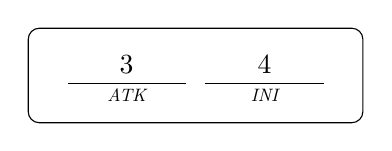
\begin{tikzpicture}[lc/.style={below,scale=0.65,font=\itshape}]
        \draw[rounded corners] (0,0) rectangle ++(4.25,1.2);
        \draw (0.5,0.5) -- ++(1.5,0) node[lc,midway] {ATK} node[above,midway] {3};
        \draw (2.25,0.5) -- ++(1.5,0) node[lc,midway] {INI} node[above,midway] {4};
    \end{tikzpicture}
\end{wrapfigure}

\def\awimp#1{\index{Charakter!Angriffswerte!#1}\imp{#1}}
\label{char:attack}\index{Charakter!Angriffswerte}Für den Angriff gibt es zwei grundlegende Werte, die \awimp{Attacke (\ability{atk})} wie auch \awimp{Initiative (\ability{ini})}.
Für letztere sind niedere Werte besser, da ein Zug bei jedem vielfachen des hochzählenden Initiativwertes ausgeführt werden darf. 
Beide Werte werden von mir festgelegt und werden auf Basis der anderen
Fertigkeiten im Folgenden berechnet\footnote{Die genaue Formel steht noch aus.}.

\paragraph{Hauptwerte}
\begin{sccenter}
    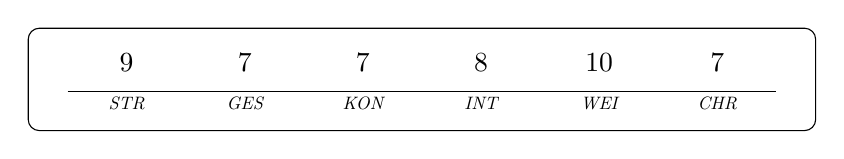
\begin{tikzpicture}[lc/.style={below,scale=0.65,font=\itshape}]
        \draw[rounded corners] (0,0) rectangle ++(10,1.3);
        \foreach[count=\i] \a/\b in {9/STR,7/GES,7/KON,8/INT,10/WEI,7/CHR} {
            \node[lc] at(1.25+1.5*\i-1.5,0.5) {\b}; 
            \node[above] at(1.25+1.5*\i-1.5,0.5) {\strut\a}; 
        }
        \draw (0.5,0.5) -- ++(9,0);
    \end{tikzpicture}
\end{sccenter}
Es gibt sechs große Werte die jeweils auf eine \dice{}{20} Probe abzielen. 

\def\hwimp#1{\index{Charakter!Hauptwerte!#1}\imp{#1}}
\index{Charakter!Hauptwerte}\label{char:strength}Wir kennen die folgenden sechs Werte: \hwimp{Stärke (\ability{str})}, \hwimp{Geschicklichkeit (\ability{ges})}, \hwimp{Konsitution (\ability{kon})}, \hwimp{Intuition (\ability{int})}, \hwimp{Weisheit (\ability{wei})}, \hwimp{Charisma (\ability{chr})}.
Alle diese Werte starten mit einer 7, zu Beginn habt ihr 6 Punkte, die
ihr \(1:1\) auf diese verteilen dürft.
Anschließend können \GP{} eingesetzt werden um die Punkte weiter zu steigern.
Dafür gelten die folgenden Kosten:
\begin{itemize}
    \item Um auf die Stufen 1 bis 11 zu gelangen, müssen je \GP[6] gezahlt werden.
    \item Um auf die Stufen 12 bis 16 zu gelangen, müssen je \GP[12] gezahlt werden.
    \item Um auf die Stufen 17 bis 19 zu gelangen, müssen je \GP[18] gezahlt werden.
\end{itemize}

\paragraph{Wahrnehmung}
\begin{wrapfigure}[4]{r}{0.175\linewidth}
    \vspace*{-0.75\topsep}\centering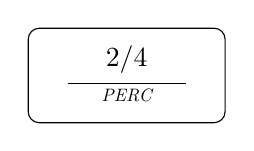
\begin{tikzpicture}[lc/.style={below,scale=0.65,font=\itshape}]
        \draw[rounded corners] (0,0) rectangle ++(2.5,1.2);
        \draw (0.5,0.5) -- ++(1.5,0) node[lc,midway] {PERC} node[above,midway] {2/{\smaller4}};
    \end{tikzpicture}
\end{wrapfigure}
Die \index{Charakter!Wahrnehmung}\imp{Wahrnehmung} ist besonders, da sie nur in vier Stufen gesteigert werden kann und keine Fertigkeit ist auf die gewürfelt wird.
Jeder startet hier mit einem Wert von 1 und kann jeweils mit \GP[4] gesteigert werden.
Je höher der Wert, desto höher ist die grundlegende Aufmerksamkeit des Charakters.
Die Stufen werden intern von mir vergeben. Ein passiver Wert kann keine aktive Probe ersetzen\footnote{Wenn man zum Beispiel eine Stelle auf Fallen überprüfen will, so muss dies durch eine Probe geschehen. Allerdings kann der passive Wert einen darauf hinweisen, dass ein Mann nach einer Waffe greift -- ohne dass man damit gerechnet hätte.}.

\subsection{Inventar}

Die genaue Umsetzung des Inventarsystems steht noch aus. Grob sagen wir, dass wir alles in der Ausrüstungs gestatten, was wir uns \say{logisch} vorstellen können. Zwölf Zelte? Eher unwahrscheinlich. Ein Zelt an den Rucksack drangepackt? Schon nachvollziehbarer. Die \link[char:strength]{Stärke} fließt mit in die Tragekapazität ein.

\subsection{Fertigkeiten}

\index{Fertigkeiten}Die Macht aller Mächte sammelt sich in den folgenden Gruppen. Um eine Fertigkeit zu steigern gibt es eine einfache Kostentabelle in vier Stufen:
\begin{itemize}
    \item Um auf die Punkte 1 bis 3 zu steigern, betragen die Kosten \SP[1].
    \item Um auf die Punkte 4 bis 6 zu steigern, betragen die Kosten \SP[2].
    \item Um auf die Punkte 7 bis 9 zu steigern, betragen die Kosten \SP[3].
    \item Um auf die Punkte 10 und höher zu steigern, betragen die Kosten \SP[4].
\end{itemize}
Es gibt keine (künstliche) Obergrenze für das Steigern der Fertigkeiten. In den folgenden Erklärungen steht in den Klammern jeweils die Anzahl der \SP, die zu Beginn zur Verfügung stehen.

\paragraph{Nahkampf (\SP[40])}

\index{Fertigkeiten!Nahkampf}Im \emph{Nahkampf} gibt es acht Kategorien auf welche die Punkte verteilt werden können: \begin{multicols}{4}
    \def\idnk#1{\index{Fertigkeiten!Nahkampf!#1}#1}%
    \begin{itemize}
        \item \idnk{Dolche}
        \item \idnk{Faustkampf}
        \item \idnk{Fechtwaffen}
        \item \idnk{Peitschen}
        \item \idnk{Schwerter}
        \item \idnk{Speere}
        \item \idnk{Stäbe}
        \item \idnk{Zweihänder}
    \end{itemize}
\end{multicols}
Auf die Kategorien wird mittels des \link[char:attack]{Attacke}-Werts direkt gewürfelt. Da nur ein Würfelwurf erfolgt ergeben die Werte hier zusammen mit dem Angriffs-Wert den Würfelwurf der im Falle eines Angriffs zu leisten ist. 
% TODO: link Fertigkeitenkompendium

\paragraph{Fernkampf (\SP[40])}

\index{Fertigkeiten!Fernkampf}Im \emph{Fernkampf} gibt es ebenfalls acht Kategorien auf die sich Punkte verteilen lassen:
\begin{multicols}{4}
    \def\idfk#1{\index{Fertigkeiten!Fernkampf!#1}#1}%
    \begin{itemize}
        \item \idfk{Armbrust}
        \item \idfk{Blasrohr}
        \item \idfk{Bogen}
        \item \idfk{Gewehre}
        \item \idfk{Granaten}
        \item \idfk{Pistolen}
        \item \idfk{Wurfmesser}
        \item \idfk{Wurfspeere}
    \end{itemize}
\end{multicols}
Auch auf diese Kategorien wird mittels des \link[char:attack]{Attacke}-Werts direkt gewürfelt.

\paragraph{Körperliches (\SP[28])}

\index{Fertigkeiten!Körperliches}Es gibt zwölf körperliche Kategorien, auf die Punkte verteilt werden können.
Auf jede der Kategorie muss gewürfelt werden. Die jeweiligen Werte sind den Fertigkeiten angefügt.
Jeder Wurf ist, wie sonst auch, mit einem \dice{}{20} durchzuführen.
\begin{multicols}{2}
    \def\idkk#1#2{\index{Fertigkeiten!Körperliches!#1 \emph{\smaller(#2)}}#1 (#2)}%
    \def\idk#1#2#3#4{\idkk{#1}{\ability{#2}, \ability{#3}, \ability{#4}}}%
    \begin{itemize}
        \item \idk{Athletik}{str}{ges}{kon}
        \item \idk{Bedrohen}{str}{str}{chr}
        \item \idk{Diebstahl}{ges}{ges}{chr}
        \item \idk{Gauklerei}{ges}{ges}{chr}
        \item \idk{Klettern}{str}{str}{kon}
        \item \idk{Körperbeherrschung}{kon}{str}{str}
        \item \idk{Reiten}{kon}{kon}{ges}
        \item \idk{Schleichen}{kon}{ges}{ges}
        \item \idk{Schwimmen}{kon}{kon}{str}
        \item \idk{Sinnesschärfe}{int}{int}{int}
        \item \idk{Tanzen}{ges}{ges}{int}
        \item \idk{Zechen}{kon}{kon}{kon}
    \end{itemize}
\end{multicols}

\paragraph{Gesellschaftliches/Soziales (\SP[16])}

\index{Fertigkeiten!Gesellschaftliches}Dieser Abschnitt zählt neun Kategorien auf die jeweils wieder mit einem \dice{}{20} geworfen wird:
\begin{multicols}{2}
    \def\idgg#1#2{\index{Fertigkeiten!Gesellschaftliches!#1 \emph{\smaller(#2)}}#1 (#2)}%
    \def\idg#1#2#3#4{\idgg{#1}{\ability{#2}, \ability{#3}, \ability{#4}}}%
    \begin{itemize}
        \item \idg{Begeistern}{chr}{chr}{int}
        \item \idg{Betören}{chr}{chr}{int}
        \item \idg{Eloquenz}{wei}{ges}{chr}
        \item \idg{Lügen}{int}{chr}{chr}
        \item \idg{Manipulieren}{str}{chr}{int}
        \item \idg{Menschenkenntnis}{wei}{int}{int}
        \item \idg{Schauspiel}{kon}{int}{chr}
        \item \idg{Selbstbeherrschung}{kon}{kon}{chr}
        \item \idg{Verkleidung}{wei}{wei}{ges}
    \end{itemize}
\end{multicols}

\paragraph{Natur und Umwelt (\SP[16])}

\index{Fertigkeiten!Natur \& Umwelt}Auch dieser Block umfasst neun Kategorien auf die mit einem \dice{}{20} geworfen wird:
\begin{multicols}{2}
    \def\idnn#1#2{\index{Fertigkeiten!Natur \& Umwelt!#1 \emph{\smaller(#2)}}#1 (#2)}%
    \def\idn#1#2#3#4{\idnn{#1}{\ability{#2}, \ability{#3}, \ability{#4}}}%
    \begin{itemize}
        \item \idn{Angeln}{str}{wei}{int}
        \item \idn{Fährtensuche}{wei}{wei}{int}
        \item \idn{Fallenstellen}{str}{wei}{int}
        \item \idn{Fesseln}{str}{str}{wei}
        \item \idn{Orientierung}{wei}{wei}{int}
        \item \idn{Pflanzenkunde}{wei}{wei}{kon}
        \item \idn{Wetterkenntnis}{int}{int}{wei}
        \item \idn{Wildnisleben}{str}{str}{int}
        \item \idn{Zähmung}{int}{int}{wis}
    \end{itemize}
\end{multicols}

\paragraph{Wissen (\SP[28])}

\index{Fertigkeiten!Wissen}Dieser Abschnitt umfasst 20 Kategorien, wobei die Kategorien \emph{Sprache} und \emph{Schrift} besonders sind. Da sie als \say{Lesen und Schreiben} Talente nicht \say{bewürfelt} werden müssen. % TODO: link

Die Kategorien \emph{Magie} und \emph{Magiekunde} unterscheidet, dass erstere praktisch (also die aktive Anwendung) und letztere eher das theoretische Wissen über die Magie bezeichnet.
\begin{multicols}{2}
    \def\idww#1#2{\index{Fertigkeiten!Wissen!#1 \emph{\smaller(#2)}}#1 (#2)}%
    \def\idw#1#2#3#4{\idww{#1}{\ability{#2}, \ability{#3}, \ability{#4}}}%
    \begin{itemize}
        \item \idw{Anatomie}{wei}{wei}{str}
        \item \idw{Astronomie}{wei}{ges}{int}
        \item \idw{Baukunst}{wei}{str}{str}
        \item \idw{Geographie}{wei}{ges}{ges}
        \item \idw{Geschichte}{wei}{kon}{kon}
        \item \idw{Gossenwissen}{wei}{ges}{kon}
        \item \idw{Kriegskunst}{wei}{str}{str}
        \item \idw{Kryptographie}{we }{int}{int}
        \item \idw{Legenden \& Sagen}{wei}{int}{chr}
        \item \idw{Magie}{wei}{wei}{wei}
        \item \idw{Magiekunde}{wei}{chr}{wei}
        \item \idw{Mathematik}{wei}{int}{wei}
        \item \idw{Mechanik}{wei}{str}{int}
        \item \idw{Philosophie}{wei}{int}{int}
        \item \idw{Rechtskunde}{wei}{chr}{chr}
        \item \idww{Schrift}{1-5}
        \item \idww{Sprache}{1-5}
        \item \idw{Sprachkunde}{wei}{chr}{chr}
        \item \idw{Steinkunde}{wei}{int}{int}
        \item \idw{Viehzucht}{wei}{int}{int}
    \end{itemize}
\end{multicols}

\paragraph{Handwerk (\SP[28])}

\index{Fertigkeiten!Handwerk}Die Handwerk umfasst 27 Kategorien auf welche die Punkte verteilt werden können. Es wird, wie überall sonst auch ein \dice{}{20} geworfen:
\begin{multicols}{2}
    \def\idhh#1#2{\index{Fertigkeiten!Handwerk!#1 \emph{\smaller(#2)}}#1 (#2)}%
    \def\idh#1#2#3#4{\idhh{#1}{\ability{#2}, \ability{#3}, \ability{#4}}}%
    \begin{itemize}
        \item \idh{Ackerbau}{kon}{str}{int}
        \item \idh{Fahrzeuge lenken}{wis}{int}{kon}
        \item \idh{Gerber}{str}{str}{int}
        \item \idh{Handel}{wei}{chr}{chr}
        \item TODO: others
    \end{itemize}
\end{multicols}

\paragraph{Gaben (\SP[16])}